\documentclass[border=10pt]{standalone}

\usepackage{tikz}
\usepackage{tikzsymbols}
\usetikzlibrary{calc,patterns,shapes.geometric}

\def\centerarc[#1](#2)(#3:#4:#5){\draw[#1] ($(#2)+({#5*cos(#3)},{#5*sin(#3)})$) arc (#3:#4:#5);}

\begin{document}
	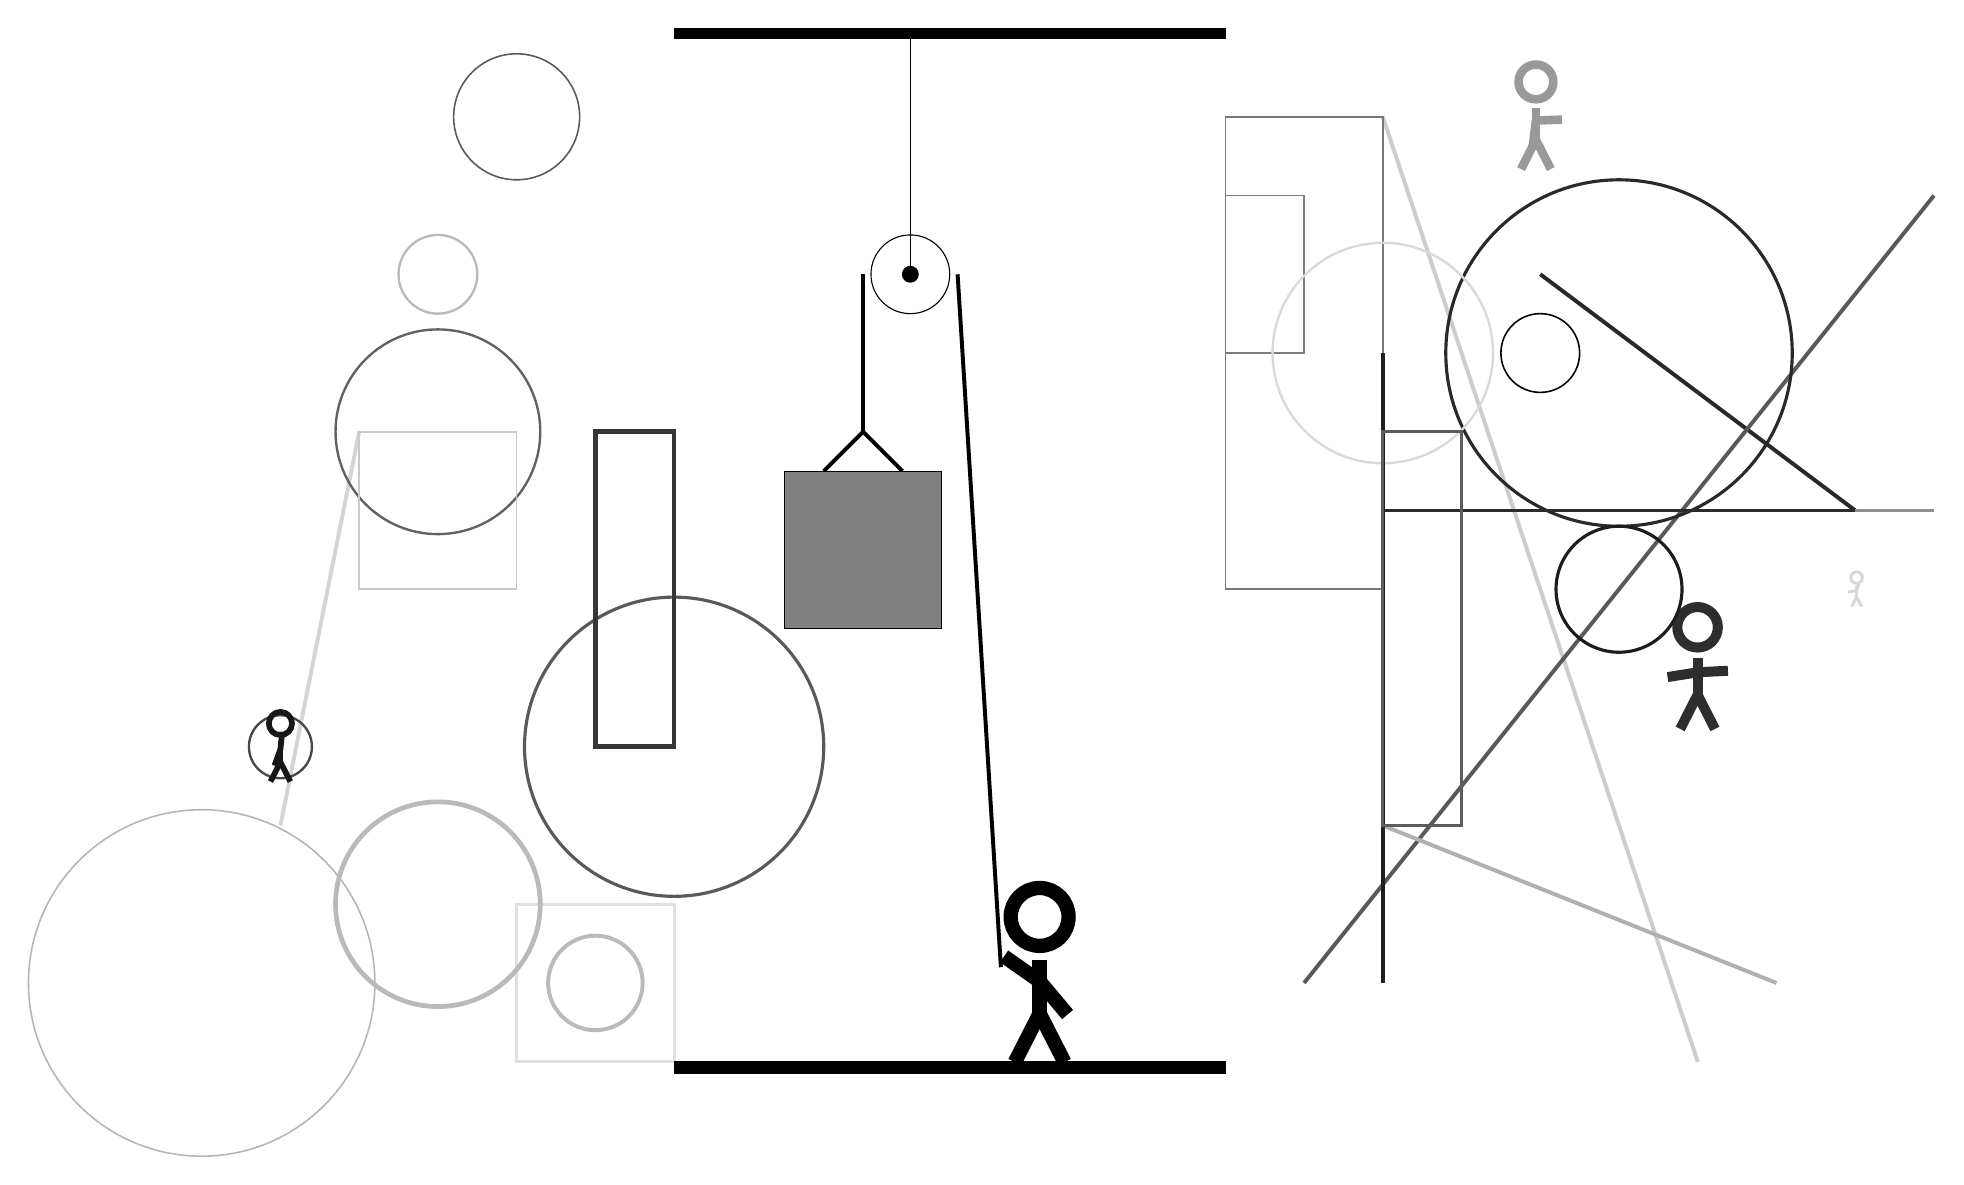
\begin{tikzpicture}
		%%%%% START %%%%%
		
		\draw[fill=black] (-2, 10) rectangle (5, 10.125);
		
		\draw[line width=0.5mm, color=black!84](9, 7) -- (13, 4);
		
		\node[line width=0.2mm, color=black!82] at (11, 2) {\Strichmaxerl[7][9][3]};
		\draw[line width=0.5mm, color=black!17](-6, 5) -- (-7, 0);
		\draw [line width=0.4mm, color=black!65](-2, 1) circle (1.9);
		\draw[line width=0.5mm, color=black!43](7, 4) -- (14, 4);
		
		\draw [line width=0.2mm, color=black!100](9, 6) circle (0.5);
		\draw [line width=0.2mm, color=black!65](-4, 9) circle (0.8);
		
		\draw[line width=0.5mm, color=black!20](7, 9) -- (11, -3);
		\draw [line width=0.3mm, color=black!72](-7, 1) circle (0.4);
		
		\node[line width=0.7mm, color=black!40] at (9, 9) {\Strichmaxerl[6][83][2]};
		
		\draw[line width=0.5mm, color=black!65](6, -2) -- (14, 8);
		
		\draw[line width=0.2mm, color=black!53] (7, 3) rectangle (5, 9);
		\draw [line width=0.4mm, color=black!84](10, 6) circle (2.2);
		
		\node[line width=0.6mm, color=black!91] at (-7, 1) {\Strichmaxerl[4][70][84]};
		\draw[line width=0.5mm, color=black!83](7, 4) -- (13, 4);
		\draw [line width=0.4mm, color=black!89](10, 3) circle (0.8);
		
		\draw[line width=0.4mm, color=black!12] (-2, -1) rectangle (-4, -3);
		\draw[line width=0.2mm, color=black!51] (6, 6) rectangle (5, 8);
		\node[line width=0.6mm, color=black!16] at (13, 3) {\Strichmaxerl[2][11][72]};
		\draw [line width=0.2mm, color=black!29](-8, -2) circle (2.2);
		\draw[line width=0.5mm, color=black!31](7, 0) -- (12, -2);
		\draw [line width=0.3mm, color=black!62](-5, 5) circle (1.3);
		\draw [line width=0.6mm, color=black!27](-5, -1) circle (1.3);
		\draw[line width=0.6mm, color=black!79] (-2, 1) rectangle (-3, 5);
		\draw [line width=0.5mm, color=black!27](-3, -2) circle (0.6);
		\draw [line width=0.3mm, color=black!15](7, 6) circle (1.4);
		
		\draw [line width=0.6mm, color=black!42](8, 1) circle (0.0);
		\draw[line width=0.2mm, color=black!21] (-4, 3) rectangle (-6, 5);
		\draw[line width=0.5mm, color=black!88](7, 6) -- (7, -2);
		\draw[line width=0.4mm, color=black!64] (7, 0) rectangle (8, 5);
		\draw [line width=0.2mm, color=black!67](10, 3) circle (0.0);
		
		\draw [line width=0.3mm, color=black!27](-5, 7) circle (0.5);
		
		\draw (1, 7) circle (0.5);
		\draw[fill=black] (1, 7) circle (0.1);
		\draw (1, 10) -- (1, 7);
		
		\draw[line width=0.5mm] (-0.1, 4.5) -- (0.4, 5.0) -- (0.9, 4.5);
		\draw[fill=black!50] (-0.6, 4.5) rectangle (1.4, 2.5);
		
		\draw[line width=0.5mm] (0.4, 7) -- (0.4, 5.0);
		\centerarc[line width=0.5mm](1, 7)(0:180:0.6);
		\draw[line width=0.5mm](1.6, 7) -- (2.15, -1.8);
		
		\node at (2.6, -1.9) {\Strichmaxerl[10][-35][-50]};
		
		\draw[fill=black] (-2, -3) rectangle (5, -3.15);
		
		%%%%% END %%%%%
	\end{tikzpicture}
\end{document}